\hypertarget{gerenciamento-de-alarmes}{%
\chapter{Gerenciamento de Alarmes}\label{gerenciamento-de-alarmes}}

\section*{Objetivos de Aprendizagem}

Ao final deste capítulo, o leitor será capaz de:

\begin{itemize}
\tightlist
\item
  Explicar por que o gerenciamento de alarmes é uma disciplina de engenharia, e não uma configuração de software.
\item
  Diferenciar alarme, evento e advertência, e distinguir prioridade de severidade.
\item
  Reconhecer o escopo de cada referência normativa: ANSI/ISA-18.2, IEC 62682, EEMUA 191 e NAMUR NA 102.
\item
  Descrever as dez etapas do ciclo de vida de gerenciamento de alarmes.
\item
  Preencher uma ficha de racionalização de alarme.
\item
  Analisar o desempenho de um sistema de alarmes a partir de métricas usuais de mercado.
\item
  Implementar um alarme simples em SCADA e em plataforma IIoT.
\end{itemize}

\begin{center}\rule{0.5\linewidth}{0.5pt}\end{center}

\hypertarget{o-problema-que-o-gerenciamento-de-alarmes-resolve}{%
\section{O problema que o gerenciamento de alarmes resolve}\label{o-problema-que-o-gerenciamento-de-alarmes-resolve}}

Um sistema de alarmes é a última linha de defesa entre uma condição anormal e um acidente. Quando funciona, o operador é avisado exatamente do que importa, no momento em que ainda pode agir. Quando não funciona, o operador recebe centenas de mensagens simultâneas e passa a ignorá-las --- ou, pior, desativa o som do sistema.

O sintoma mais conhecido é a \textbf{inundação de alarmes} (\emph{alarm flood}): uma perturbação de processo dispara, em poucos segundos, um número de alarmes maior do que um operador consegue ler e processar.

\begin{caixaatencao}

\textbf{Atenção:} A inundação de alarmes não é consequência de ``operador desatento''. É consequência de projeto: alarmes criados sem critério, limites copiados do valor de projeto, ausência de \emph{deadband} e de atraso de confirmação, e nenhuma racionalização. O operador é a vítima, não a causa.

\end{caixaatencao}

Alguns efeitos medíveis de um sistema de alarmes mal projetado:

\begin{itemize}
\tightlist
\item
  \textbf{Perda de priorização:} se 80\% dos alarmes são ``críticos'', nenhum é crítico.
\item
  \textbf{Cegueira por ruído:} alarmes repetitivos (\emph{chattering}) escondem o alarme novo.
\item
  \textbf{Fadiga de decisão:} cada mensagem irrelevante reduz a capacidade de julgamento.
\item
  \textbf{Desconfiança do sistema:} o operador passa a silenciar (\emph{shelve}) em massa, e a proteção desaparece.
\item
  \textbf{Perda de rastreabilidade:} sem registro consistente, não há como investigar o incidente depois.
\end{itemize}

\begin{caixafigura}

\textbf{{[}Figura 10.1 -- Inundação de alarmes: painel de alarmes antes e depois da racionalização{]}}
\emph{Lado esquerdo: lista com dezenas de alarmes ativos no mesmo segundo, todos em vermelho, sem ordem de prioridade visível. Lado direito: a mesma perturbação com dez alarmes, ordenados por prioridade, com o alarme de causa raiz destacado. Usar captura de tela genérica de um painel de alarmes; não usar marca de fabricante.}

\end{caixafigura}

\begin{center}\rule{0.5\linewidth}{0.5pt}\end{center}

\hypertarget{conceitos-e-taxonomia}{%
\section{Conceitos e taxonomia}\label{conceitos-e-taxonomia}}

A primeira dificuldade prática é terminológica: em muitos projetos, ``alarme'', ``evento'' e ``aviso'' são usados como sinônimos. Não são.

\textbf{Tabela 10.1 -- Termos essenciais de gerenciamento de alarmes}

\begin{longtable}[]{@{}
  >{\raggedright\arraybackslash}p{(\columnwidth - 4\tabcolsep) * \real{0.3333}}
  >{\raggedright\arraybackslash}p{(\columnwidth - 4\tabcolsep) * \real{0.3333}}
  >{\raggedright\arraybackslash}p{(\columnwidth - 4\tabcolsep) * \real{0.3333}}@{}}
\toprule\noalign{}
\begin{minipage}[b]{\linewidth}\raggedright
Termo
\end{minipage} & \begin{minipage}[b]{\linewidth}\raggedright
Definição
\end{minipage} & \begin{minipage}[b]{\linewidth}\raggedright
Exemplo
\end{minipage} \\
\midrule\noalign{}
\endhead
\bottomrule\noalign{}
\endlastfoot
\textbf{Evento} & Qualquer mudança de estado registrada pelo sistema & Bomba ligada; operador entrou no sistema \\
\textbf{Alarme} & Evento que exige \textbf{resposta do operador} dentro de um tempo definido & Alta temperatura do mancal acima de 85 \ensuremath{^\circ}C \\
\textbf{Advertência} (\emph{alert}) & Informação que não exige resposta imediata, mas pede atenção & Filtro com 70\% de saturação \\
\textbf{Supressão} (\emph{suppression}) & Ocultação temporária por projeto, enquanto a causa está ativa & Alarmes de nível suprimidos durante enchimento \\
\textbf{Silenciamento temporário} (\emph{shelving}) & Ocultação manual, com prazo e justificativa & Alarme em manutenção por 4 h \\
\textbf{Alarme fixo} (\emph{standing}) & Permanece ativo por longos períodos sem ação possível & Falha de sensor não reparado \\
\textbf{Alarme obsoleto} (\emph{stale}) & Não é atualizado ou não é limpo por falha de configuração & Alarme ativo cuja condição já cessou \\
\end{longtable}

A definição operacional de alarme tem duas partes que não podem ser separadas: \textbf{existe uma resposta possível} e \textbf{existe tempo para executá-la}. Se não há ação a tomar, não é alarme --- é registro. Se o operador tem 30 segundos para agir e a tela mostra o alarme em uma página que ele abre em 40 segundos, também não é alarme: é informação histórica.

\hypertarget{prioridade-e-severidade-nuxe3o-suxe3o-a-mesma-coisa}{%
\subsection{Prioridade e severidade não são a mesma coisa}\label{prioridade-e-severidade-nuxe3o-suxe3o-a-mesma-coisa}}

Essa confusão aparece em quase toda especificação de SCADA.

\begin{itemize}
\tightlist
\item
  \textbf{Severidade} descreve a \textbf{consequência} da condição anormal: o que acontece se ninguém agir.
\item
  \textbf{Prioridade} descreve a \textbf{urgência da resposta} do operador: em quanto tempo ele precisa agir.
\end{itemize}

Uma falha de instrumento pode ter consequência alta (perde-se a medição de vazão de um reator) e urgência baixa (há redundância e o processo continua seguro por horas). Prioridade alta, portanto, não é sinônimo de ``coisa grave'': é ``aja agora''.

\textbf{Tabela 10.2 -- Matriz usual de prioridade por tempo de resposta}

\begin{longtable}[]{@{}
  >{\raggedright\arraybackslash}p{(\columnwidth - 4\tabcolsep) * \real{0.3333}}
  >{\raggedright\arraybackslash}p{(\columnwidth - 4\tabcolsep) * \real{0.3333}}
  >{\raggedright\arraybackslash}p{(\columnwidth - 4\tabcolsep) * \real{0.3333}}@{}}
\toprule\noalign{}
\begin{minipage}[b]{\linewidth}\raggedright
Prioridade
\end{minipage} & \begin{minipage}[b]{\linewidth}\raggedright
Tempo de resposta esperado
\end{minipage} & \begin{minipage}[b]{\linewidth}\raggedright
Referência de apresentação
\end{minipage} \\
\midrule\noalign{}
\endhead
\bottomrule\noalign{}
\endlastfoot
Crítica & Segundos a poucos minutos & Destaque máximo, som distinto, exige reconhecimento \\
Alta & Minutos & Destaque visual forte, som padrão \\
Média & Dezenas de minutos & Destaque visual moderado \\
Baixa & Horas ou próximo turno & Apenas registro em lista, sem som \\
\end{longtable}

A distribuição de prioridades também é um critério de qualidade: em um sistema maduro, a maior parte dos alarmes é de prioridade baixa e média, e a prioridade crítica é rara. Um sistema em que metade dos alarmes é crítica está mal priorizado, por definição.

\begin{caixadica}

\textbf{Dica:} antes de discutir prioridade, responda por escrito, para cada alarme: \emph{``qual é a ação esperada do operador e em quanto tempo ela precisa começar?''} Alarmes que não sobrevivem a essa pergunta são candidatos a remoção, não a reclassificação.

\end{caixadica}

\hypertarget{ajustes-que-definem-o-comportamento}{%
\subsection{Ajustes que definem o comportamento}\label{ajustes-que-definem-o-comportamento}}

Três parâmetros determinam se um alarme é útil ou ruído:

\begin{itemize}
\tightlist
\item
  \textbf{Limite} (\emph{setpoint}): valor que dispara a condição.
\item
  \textbf{Faixa morta} (\emph{deadband}): diferença necessária para limpar o alarme, evitando oscilação em torno do limite.
\item
  \textbf{Atraso de confirmação} (\emph{on-delay}): tempo que a condição precisa persistir para que o alarme seja gerado. Elimina disparos fugazes (\emph{fleeting}) causados por transitórios de partida.
\end{itemize}

\begin{caixafigura}

\textbf{{[}Figura 10.2 -- Limite, faixa morta e atraso de confirmação{]}}
\emph{Gráfico de tendência com a variável cruzando o limite três vezes em poucos segundos. Marcar: (a) disparo no cruzamento com atraso de 3 s; (b) zona de faixa morta impedindo o disparo/limpeza repetitivo; (c) os alarmes que existiriam sem esses ajustes, em linha tracejada. Incluir eixo de tempo legível.}

\end{caixafigura}

\begin{center}\rule{0.5\linewidth}{0.5pt}\end{center}

\hypertarget{normas-e-o-escopo-de-cada-uma}{%
\section{Normas e o escopo de cada uma}\label{normas-e-o-escopo-de-cada-uma}}

Quatro referências dominam o assunto, e elas \textbf{não são equivalentes}.

\textbf{Tabela 10.3 -- Comparação das referências normativas}

\begin{longtable}[]{@{}
  >{\raggedright\arraybackslash}p{(\columnwidth - 4\tabcolsep) * \real{0.3333}}
  >{\raggedright\arraybackslash}p{(\columnwidth - 4\tabcolsep) * \real{0.3333}}
  >{\raggedright\arraybackslash}p{(\columnwidth - 4\tabcolsep) * \real{0.3333}}@{}}
\toprule\noalign{}
\begin{minipage}[b]{\linewidth}\raggedright
Referência
\end{minipage} & \begin{minipage}[b]{\linewidth}\raggedright
Natureza
\end{minipage} & \begin{minipage}[b]{\linewidth}\raggedright
Escopo e uso típico
\end{minipage} \\
\midrule\noalign{}
\endhead
\bottomrule\noalign{}
\endlastfoot
\textbf{ANSI/ISA-18.2} & Norma (ISA) & Gerenciamento de alarmes na indústria de processo; define o ciclo de vida; edição vigente de 2016 (a primeira é de 2009) \\
\textbf{IEC 62682} & Norma (IEC) & Mesmo escopo em base internacional, alinhada à ISA-18.2; edição vigente de \textbf{2022}, que substitui a de 2014 \\
\textbf{EEMUA 191} & Guia de engenharia (EEMUA) & Projeto, gestão e contratação de sistemas de alarme; traz valores de referência de desempenho; 3ª edição, 2013 \\
\textbf{NAMUR NA 102} & Recomendação (NAMUR) & Gerenciamento de alarmes na indústria química e farmacêutica; publicada em 2003, referência histórica que influenciou as normas \\
\end{longtable}

Notas de uso, verificadas na documentação pública dos organismos:

\begin{itemize}
\tightlist
\item
  ISA-18.2 e IEC 62682 são \textbf{quase idênticas} --- a versão IEC foi modificada a partir da ISA. Como normas, dizem \textbf{o que} deve existir em um programa de gerenciamento de alarmes, não \textbf{como} fazer.
\item
  EEMUA 191 é um \textbf{guia}, não uma norma: cobre parcialmente o ``como'' e é muito usada como referência de desempenho.
\item
  A série de \textbf{relatórios técnicos ISA-18.2} (sete documentos, alinhados à norma) aprofunda o ``como'' em cada etapa.
\item
  ISA-18.2 foi escrita para \textbf{não conflitar} com EEMUA 191 e NAMUR NA 102: o objetivo foi criar terminologia e atividades consistentes entre as referências.
\end{itemize}

\begin{caixanota}

\textbf{Atualização tecnológica:} o conceito de gerenciamento de alarmes não muda com IIoT --- muda o \textbf{alcance}. Em SCADA clássico, os alarmes vivem no servidor de supervisão. Em arquiteturas atuais, plataformas IIoT possuem entidade de alarme própria (por exemplo, o tipo \emph{alarm} do ThingsBoard, com severidade, estado e detalhes) e podem gerar alarmes na borda, antes da nuvem. A disciplina (filosofia, racionalização, prioridade, monitoramento) permanece a mesma.

\end{caixanota}

\begin{caixaatencao}

\textbf{Atenção:} não atribua requisitos de ISA-18.2/IEC 62682 a normas de outra família, como \textbf{IEC 60839} (alarme de segurança eletrônica/patrimonial e sistemas de detecção de intrusão) ou a normas de detecção e alarme de incêndio. São escopos distintos: alarme de \textbf{processo} exige resposta de operador sobre uma variável de processo; alarme de \textbf{segurança patrimonial} trata de detecção de intrusão. Se o material antigo do curso fizer essa associação, corrija e explique a diferença.

\end{caixaatencao}

\begin{center}\rule{0.5\linewidth}{0.5pt}\end{center}

\hypertarget{ciclo-de-vida}{%
\section{Ciclo de vida}\label{ciclo-de-vida}}

Normas e guias organizam o trabalho em etapas. O ciclo é iterativo: a saída da auditoria alimenta a filosofia.

\begin{center}
\IfFileExists{../figuras/capitulo-10-m1.pdf}{%
  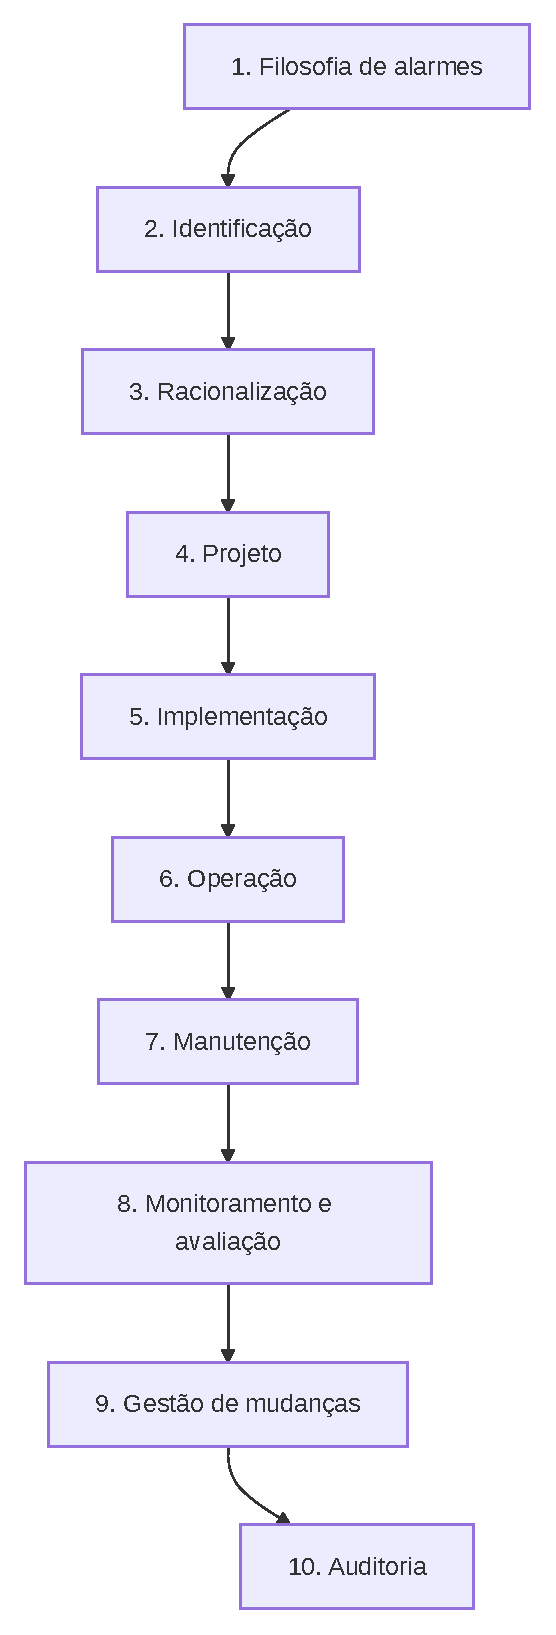
\includegraphics[width=\linewidth,height=0.8\textheight,keepaspectratio]{../figuras/capitulo-10-m1.pdf}%
}{\fbox{\parbox{0.9\linewidth}{\small Diagrama Mermaid ainda não renderizado: capitulo-10-m1. Rode scripts/render-mermaid.sh.}}}
\end{center}

\textbf{Tabela 10.4 -- O que cada etapa entrega}

\begin{longtable}[]{@{}
  >{\raggedright\arraybackslash}p{(\columnwidth - 4\tabcolsep) * \real{0.3333}}
  >{\raggedright\arraybackslash}p{(\columnwidth - 4\tabcolsep) * \real{0.3333}}
  >{\raggedright\arraybackslash}p{(\columnwidth - 4\tabcolsep) * \real{0.3333}}@{}}
\toprule\noalign{}
\begin{minipage}[b]{\linewidth}\raggedright
Etapa
\end{minipage} & \begin{minipage}[b]{\linewidth}\raggedright
Pergunta que responde
\end{minipage} & \begin{minipage}[b]{\linewidth}\raggedright
Produto
\end{minipage} \\
\midrule\noalign{}
\endhead
\bottomrule\noalign{}
\endlastfoot
Filosofia & Quais são os princípios, papéis e critérios de desempenho? & Documento de filosofia de alarmes \\
Identificação & Que condições precisam de alarme? & Lista de eventos candidatos \\
Racionalização & Cada alarme é necessário, único e acionável? & Ficha de racionalização por alarme \\
Projeto & Como o alarme se apresenta e se comporta? & Especificação de limite, prioridade, deadband, atraso \\
Implementação & Está configurado como especificado? & Alarmes configurados e testados \\
Operação & O operador consegue responder? & Rotina de operação e tratamento de shelving \\
Manutenção & O sistema continua íntegro? & Correção de alarmes fixos, obsoletos e falhas \\
Monitoramento e avaliação & O desempenho é adequado? & Relatórios de métricas \\
Gestão de mudanças & A alteração está justificada e registrada? & Registro de mudança aprovado \\
Auditoria & O programa funciona como previsto? & Relatório de auditoria e plano de ação \\
\end{longtable}

\begin{caixadica}

\textbf{Dica:} a etapa que separa plantas maduras das demais é a de \textbf{gestão de mudanças}. Mudar um limite de alarme é alterar um projeto: precisa de justificativa, aprovação e registro. Sem esse controle, o sistema degrada em poucos meses --- é o chamado \emph{drift} de configuração.

\end{caixadica}

\begin{center}\rule{0.5\linewidth}{0.5pt}\end{center}

\hypertarget{racionalizauxe7uxe3o-na-pruxe1tica}{%
\section{Racionalização na prática}\label{racionalizauxe7uxe3o-na-pruxe1tica}}

Racionalizar é documentar, alarme por alarme, por que ele existe e o que o operador deve fazer. A saída é uma ficha (no jargão em inglês, \emph{Alarm Basis Form} ou \emph{rationalization record}).

\textbf{Tabela 10.5 -- Campos de uma ficha de racionalização}

\begin{longtable}[]{@{}
  >{\raggedright\arraybackslash}p{(\columnwidth - 2\tabcolsep) * \real{0.5000}}
  >{\raggedright\arraybackslash}p{(\columnwidth - 2\tabcolsep) * \real{0.5000}}@{}}
\toprule\noalign{}
\begin{minipage}[b]{\linewidth}\raggedright
Campo
\end{minipage} & \begin{minipage}[b]{\linewidth}\raggedright
Conteúdo
\end{minipage} \\
\midrule\noalign{}
\endhead
\bottomrule\noalign{}
\endlastfoot
Identificação & Tag do instrumento, descrição e tipo de alarme \\
Causa & O que provoca a condição anormal \\
Consequência & O que acontece se ninguém agir (e em quanto tempo) \\
Ação esperada & O que o operador deve fazer, em passos objetivos \\
Tempo de resposta & Tempo disponível para agir \\
Prioridade & Derivada da consequência e do tempo \\
Limite, deadband e atraso & Valores justificados por processo, não copiados do projeto \\
Classificação & Prioridade, tipo (alarme/trip) e agrupamento na tela \\
Responsável e revisão & Quem aprovou e quando revalidar \\
\end{longtable}

Um teste rápido de qualidade: se a coluna ``ação esperada'' está vazia ou diz ``verificar o processo'', o alarme ainda não foi racionalizado.

\hypertarget{um-exemplo-completo}{%
\subsection{Um exemplo completo}\label{um-exemplo-completo}}

Considere um alarme de \textbf{alta temperatura} no mancal de uma bomba de processo.

\begin{itemize}
\tightlist
\item
  \textbf{Causa:} perda de lubrificação, desalinhamento ou falha de resfriamento.
\item
  \textbf{Consequência:} desgaste acelerado e falha do mancal em dezenas de minutos; parada não programada.
\item
  \textbf{Ação esperada:} verificar vazamento de óleo, checar vibração, avaliar acionamento da bomba reserva.
\item
  \textbf{Prioridade:} alta (há tempo de minutos, mas a ação é obrigatória).
\item
  \textbf{Limite:} 85 \ensuremath{^\circ}C; \textbf{deadband:} 5 \ensuremath{^\circ}C; \textbf{atraso:} 5 s.
\item
  \textbf{Justificativa:} a faixa normal é 45--70 \ensuremath{^\circ}C; 85 \ensuremath{^\circ}C indica perda de lubrificação; o \emph{deadband} evita alternância de estado perto do limite; o atraso elimina a leitura espúria de partida.
\end{itemize}

\begin{center}
\IfFileExists{../figuras/capitulo-10-m2.pdf}{%
  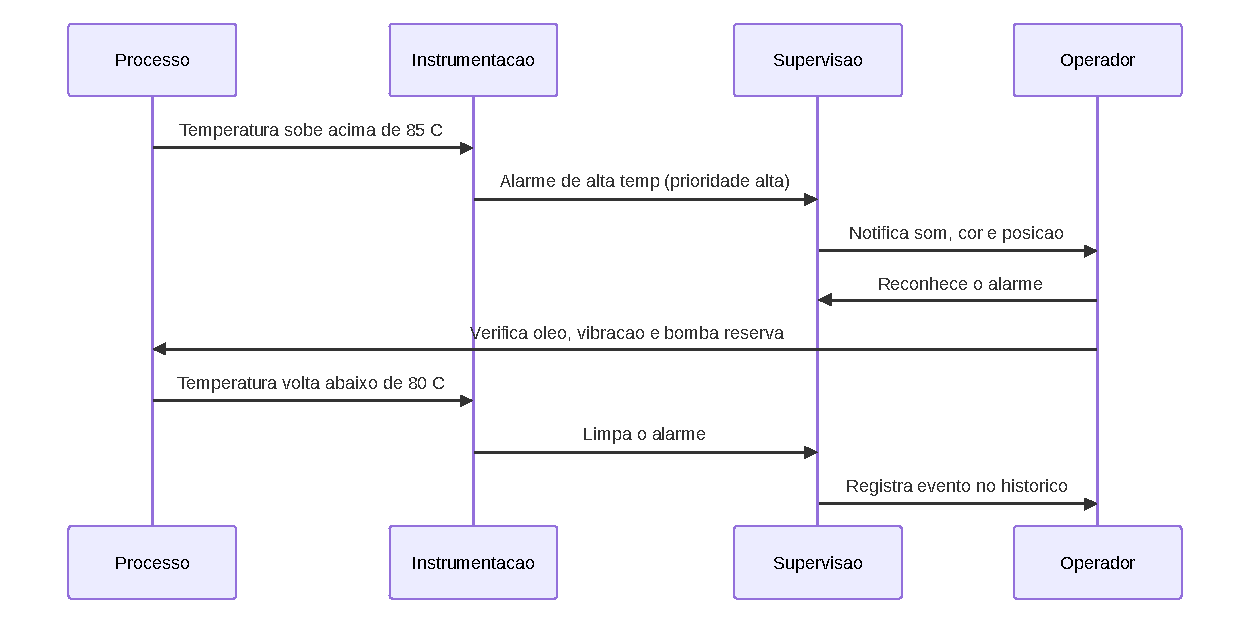
\includegraphics[width=\linewidth,height=0.8\textheight,keepaspectratio]{../figuras/capitulo-10-m2.pdf}%
}{\fbox{\parbox{0.9\linewidth}{\small Diagrama Mermaid ainda não renderizado: capitulo-10-m2. Rode scripts/render-mermaid.sh.}}}
\end{center}

\begin{figure}
\centering
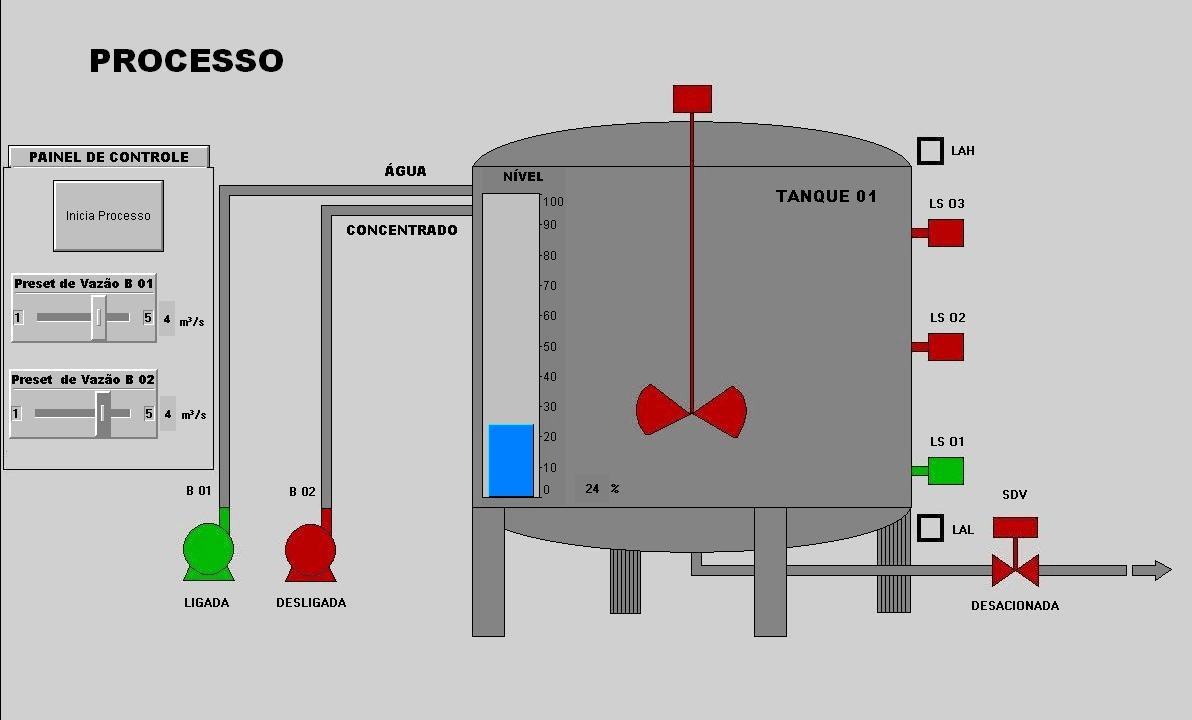
\includegraphics{../figuras/cap10-sinotico-alarmes.png}
\caption[Figura 10.3 -- Sinalização de estado no sinótico, com o alarme fora da tela de processo]{Figura 10.3 -- Sinalização de estado no sinótico, com o alarme fora da tela de processo. \textbf{Fonte:} \emph{Livro SCADA --- versão para análise}, p.~135 (Machado, Pontes e Vianna, reproduzida com crédito).}
\end{figure}

A tela separa três coisas que não podem se misturar: o \textbf{sinótico} com o estado do equipamento
(cor e forma das válvulas, altura do nível), o \textbf{painel de controle} com os \emph{setpoints} e os
indicadores de estado discreto (LAH, LS-01 a LS-03) e a \textbf{barra de navegação} que leva à lista de
alarmes. O alarme não é anunciado dentro do desenho do processo; ele recebe uma tela própria, com
horário, prioridade e botão de reconhecimento --- a separação que a Seção 10.6 justifica.

\begin{center}\rule{0.5\linewidth}{0.5pt}\end{center}

\hypertarget{apresentauxe7uxe3o-ao-operador-e-desempenho}{%
\section{Apresentação ao operador e desempenho}\label{apresentauxe7uxe3o-ao-operador-e-desempenho}}

\hypertarget{como-o-alarme-chega-ao-operador}{%
\subsection{Como o alarme chega ao operador}\label{como-o-alarme-chega-ao-operador}}

A ergonomia de telas e a sinalização de alarmes são tratadas pela \textbf{ISA-101} (\emph{Human-Machine Interfaces for Process Automation Systems}), a principal referência global para o projeto de \textbf{IHM e SCADA de alta performance}. Ela está no material de origem desta apostila (inclui o simpósio ISA-101 realizado em São Paulo, com aplicação em saneamento).

\begin{caixanota}

\textbf{Nota:} a ISA-101 \textbf{não é um software SCADA}. É um conjunto de diretrizes e padrões de engenharia para criar telas eficientes: o pacote de supervisão é escolhido à parte, e a norma diz \textbf{como} a informação deve ser apresentada ao operador. Comprar um SCADA não garante uma IHM de alta performance --- projetá-la, sim.

\end{caixanota}

O que define uma IHM/SCADA de \textbf{alta performance} pela ISA-101:

\begin{itemize}
\tightlist
\item
  \textbf{Foco cognitivo:} elimina poluição visual, gráficos 3-D excessivos e cores chamativas sem função. Cada elemento que sobra compete com o que importa.
\item
  \textbf{Uso estratégico de cores:} o processo em condição normal é desenhado em tons neutros (fundo cinza/apagado), e as cores vibrantes ficam reservadas para alarmes e anomalias. Se tudo é colorido, nada se destaca.
\item
  \textbf{Hierarquia da informação:} as telas são organizadas em níveis navegáveis, para que o operador entenda o problema rapidamente sem se perder em excesso de dados --- a hierarquia de níveis 1 a 4 detalhada no Capítulo 11.
\item
  \textbf{Tomada de decisão rápida:} é o resultado dos três itens anteriores --- reduz o tempo de resposta a situações anormais e amplia a \textbf{consciência situacional} do operador.
\end{itemize}

O gerenciamento de alarmes tratado nas Seções 10.1 a 10.5 é o outro lado da mesma moeda: a ISA-101 cuida de \textbf{como} a informação chega ao operador, enquanto a ISA-18.2 e a IEC 62682 definem \textbf{quando} um alarme deve existir.

Aplicando esses princípios à tela de alarmes:

\begin{itemize}
\tightlist
\item
  \textbf{Cor com significado único:} vermelho para prioridade crítica, âmbar para média, ciano/azul para informação. Nunca usar vermelho para decoração.
\item
  \textbf{Posição estável:} a lista de alarmes não deve reordenar a cada segundo; quem reordena esconde o alarme novo.
\item
  \textbf{Som distinto por prioridade}, com silenciamento temporário e auditável.
\item
  \textbf{Agrupamento:} a tela precisa indicar a \textbf{área} afetada, não apenas a tag.
\item
  \textbf{Taxa de atualização coerente} com a dinâmica do processo --- atualizar 10 vezes por segundo um valor que muda por hora só consome rede e desvia atenção.
\end{itemize}

\hypertarget{muxe9tricas-de-desempenho}{%
\subsection{Métricas de desempenho}\label{muxe9tricas-de-desempenho}}

O acompanhamento é o que dá objetividade à discussão. As métricas mais usadas:

\textbf{Tabela 10.6 -- Métricas usuais e valores de referência citados}

\begin{longtable}[]{@{}
  >{\raggedright\arraybackslash}p{(\columnwidth - 4\tabcolsep) * \real{0.3333}}
  >{\raggedright\arraybackslash}p{(\columnwidth - 4\tabcolsep) * \real{0.3333}}
  >{\raggedright\arraybackslash}p{(\columnwidth - 4\tabcolsep) * \real{0.3333}}@{}}
\toprule\noalign{}
\begin{minipage}[b]{\linewidth}\raggedright
Métrica
\end{minipage} & \begin{minipage}[b]{\linewidth}\raggedright
Como se lê
\end{minipage} & \begin{minipage}[b]{\linewidth}\raggedright
Referência usualmente citada
\end{minipage} \\
\midrule\noalign{}
\endhead
\bottomrule\noalign{}
\endlastfoot
Taxa média de alarmes & Alarmes por hora por operador & Máximo da ordem de 10 alarmes a cada 10 minutos \\
Volume diário & Alarmes por dia por operador & Cerca de 150 alarmes/dia como meta de sistema maduro \\
Alarmes repetitivos & Percentual que chattering & Pequena fração do total; reduzir com deadband e atraso \\
Alarmes fixos & Ativos por mais de 24 h & Tendência a zero \\
Distribuição por prioridade & Fração de críticos & Críticos como minoria clara do total \\
Tempo de resposta & Intervalo entre alarme e ação & Compatível com o tempo de resposta definido na ficha \\
\end{longtable}

\begin{caixanota}

\textbf{Nota:} esses valores são referências de mercado difundidas por EEMUA 191 e ISA-18.2. Antes de usá-los em contrato ou relatório, \textbf{verifique a redação vigente da edição atual} da referência escolhida --- a redação e a apresentação das metas mudam entre edições, e a norma não deve ser citada por aquilo que ela não afirma.

\end{caixanota}

\begin{center}\rule{0.5\linewidth}{0.5pt}\end{center}

\hypertarget{alarmes-em-scada-e-em-plataformas-iiot}{%
\section{Alarmes em SCADA e em plataformas IIoT}\label{alarmes-em-scada-e-em-plataformas-iiot}}

\hypertarget{no-scada-cluxe1ssico}{%
\subsection{No SCADA clássico}\label{no-scada-cluxe1ssico}}

O servidor de supervisão mantém o motor de alarmes:

\begin{itemize}
\tightlist
\item
  Avaliação cíclica dos limites, com deadband e atraso por tag.
\item
  Estado por alarme: ativo/não reconhecido, reconhecido, limpo, suprimido, silenciado, fora de serviço.
\item
  Registro em base de dados de eventos, com \textbf{timestamp de origem} e \textbf{timestamp de detecção} distintos --- a diferença entre eles é um dado de engenharia valioso.
\item
  Área de auditoria: quem reconheceu, quem silenciou, quem alterou limite, quando e por quê.
\end{itemize}

\begin{figure}
\centering
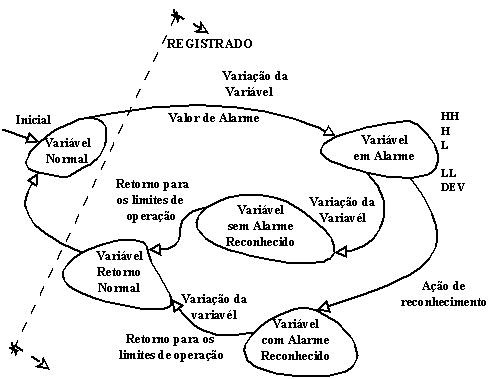
\includegraphics{../figuras/cap10-estados-alarme.png}
\caption[Figura 10.4 -- Diagrama de estados de uma variável de alarme]{Figura 10.4 -- Diagrama de estados de uma variável de alarme. \textbf{Fonte:} \emph{Livro SCADA --- versão para análise}, p.~61 (Machado, Pontes e Vianna, reproduzida com crédito).}
\end{figure}

Este é o modelo de estados do alarme, e ele explica por que \textbf{reconhecer} e \textbf{normalizar} não
são a mesma coisa. A variável parte de \emph{Normal}, entra em \emph{alarme} ao cruzar o limite e passa a
\emph{alarme reconhecido} quando o operador age. Se a condição persistir, ela \textbf{volta} ao estado de
alarme --- agora com o reconhecimento registrado. Só o retorno da variável aos limites de operação
devolve o estado \emph{normal}. Um sistema que oferece apenas ``alarme ativo/inativo'' perde essa
distinção e não consegue auditar quem agiu, quando e sobre qual condição.

\begin{figure}
\centering
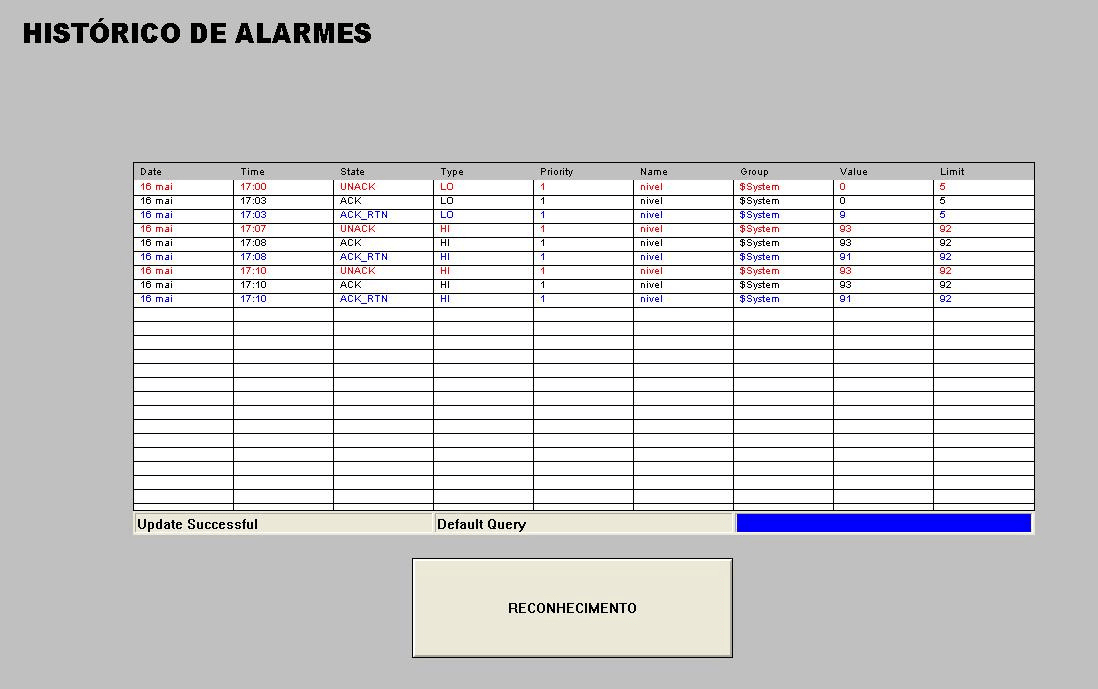
\includegraphics{../figuras/cap10-historico-alarmes.png}
\caption[Figura 10.5 -- Registro de eventos de alarme com estado, prioridade, valor e limite]{Figura 10.5 -- Registro de eventos de alarme com estado, prioridade, valor e limite. \textbf{Fonte:} \emph{Livro SCADA --- versão para análise}, p.~116 (Machado, Pontes e Vianna, reproduzida com crédito).}
\end{figure}

A janela de histórico é o lado do sistema que \textbf{não} é apagado pelo reconhecimento. As colunas
são as da ficha de racionalização transformadas em dado: \emph{state} (UNACK/ACK/RTN), \emph{type}, \emph{priority},
\emph{name}, \emph{group}, \emph{value}, \emph{limit}. Repare no botão de reconhecimento separado da consulta: quem
consulta é auditoria, quem reconhece é operação --- e as duas ações exigem perfis de acesso
diferentes.

\begin{caixaatencao}

\textbf{Atenção:} alarme gerado a partir de dado com qualidade ruim (\emph{bad quality}) é uma armadilha frequente. Se o valor é inválido por falha de comunicação, o sistema não deve gerar ``temperatura baixa'' --- deve gerar \textbf{falha de comunicação}. Tratar qualidade de dado como dado é uma das causas mais comuns de alarmes espúrios.

\end{caixaatencao}

\hypertarget{na-borda-e-na-plataforma}{%
\subsection{Na borda e na plataforma}\label{na-borda-e-na-plataforma}}

Em arquiteturas com MQTT e plataformas IIoT, o alarme pode ser gerado em três lugares: no CLP (intertravamento e proteção), no \emph{gateway} de borda (primeira avaliação de limites) e na plataforma (correlação, notificação, acompanhamento e relatório).

No ThingsBoard, o alarme é uma \textbf{entidade} com tipo, severidade e estado (\emph{active unacknowledged}, reconhecido, limpo), criada e encerrada por nós de uma \emph{rule chain}. Os campos observáveis na documentação oficial incluem tipo, severidade, origem, instante de início e de fim, estado de reconhecimento e um campo de detalhes com valores do momento.

\begin{center}
\IfFileExists{../figuras/capitulo-10-m3.pdf}{%
  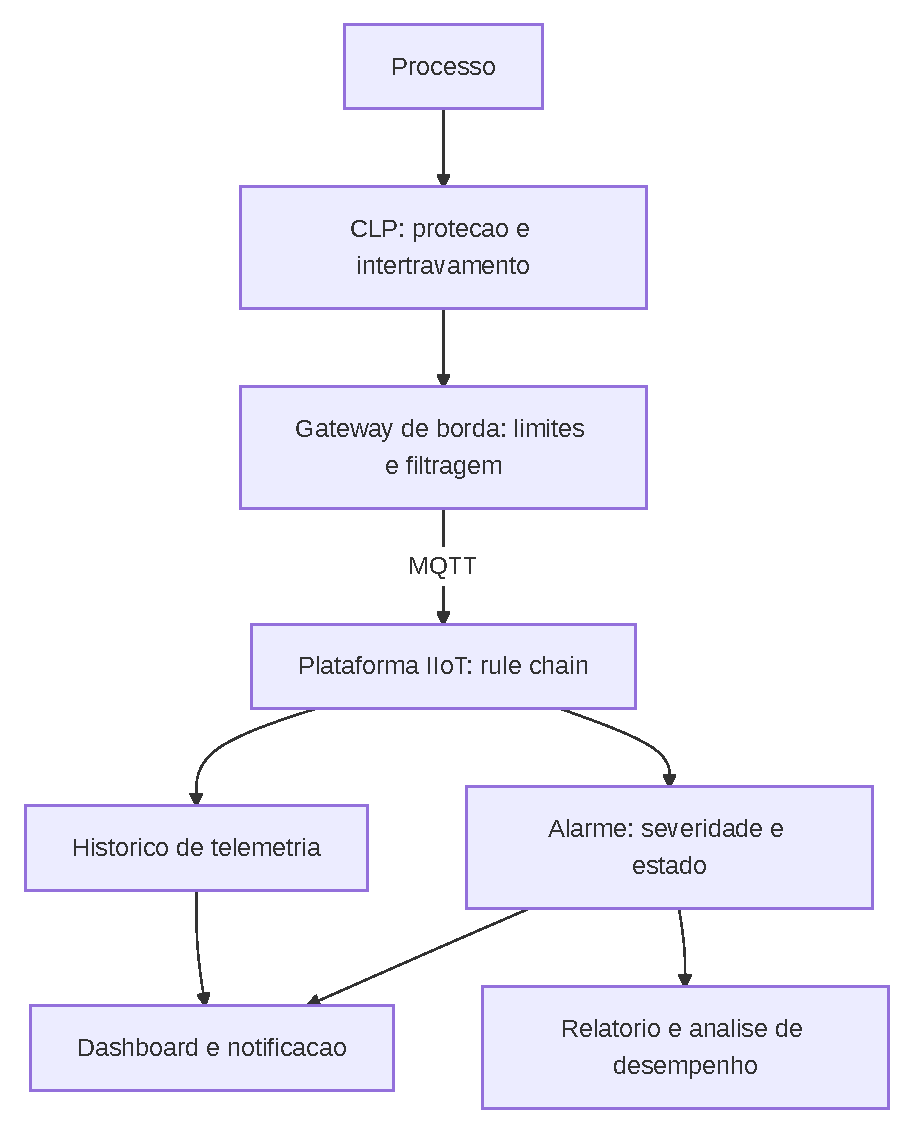
\includegraphics[width=\linewidth,height=0.8\textheight,keepaspectratio]{../figuras/capitulo-10-m3.pdf}%
}{\fbox{\parbox{0.9\linewidth}{\small Diagrama Mermaid ainda não renderizado: capitulo-10-m3. Rode scripts/render-mermaid.sh.}}}
\end{center}

A divisão de responsabilidade recomendada:

\begin{longtable}[]{@{}
  >{\raggedright\arraybackslash}p{(\columnwidth - 4\tabcolsep) * \real{0.3333}}
  >{\raggedright\arraybackslash}p{(\columnwidth - 4\tabcolsep) * \real{0.3333}}
  >{\raggedright\arraybackslash}p{(\columnwidth - 4\tabcolsep) * \real{0.3333}}@{}}
\toprule\noalign{}
\begin{minipage}[b]{\linewidth}\raggedright
Onde
\end{minipage} & \begin{minipage}[b]{\linewidth}\raggedright
O que faz
\end{minipage} & \begin{minipage}[b]{\linewidth}\raggedright
Nunca deve fazer
\end{minipage} \\
\midrule\noalign{}
\endhead
\bottomrule\noalign{}
\endlastfoot
CLP & Proteção, intertravamento, trip & Depender da rede para segurança \\
Borda & Filtragem, agregação, alarme local & Assumir lógica de segurança funcional \\
Plataforma & Correlação, notificação, histórico, relatório & Ser o único caminho para uma ação crítica \\
SCADA & Supervisão e comando do operador & Ser o único repositório de eventos \\
\end{longtable}

\begin{center}\rule{0.5\linewidth}{0.5pt}\end{center}

\hypertarget{estudo-de-caso-alarmes-de-uma-estauxe7uxe3o-de-bombeamento}{%
\section{\texorpdfstring{Estudo de caso --- alarmes de uma estação de bombeamento}{Estudo de caso  alarmes de uma estação de bombeamento}}\label{estudo-de-caso-alarmes-de-uma-estauxe7uxe3o-de-bombeamento}}

\textbf{Cenário.} Estação com quatro bombas, uma em operação e três em espera, controlando vazão para um reservatório a 12 km. Instrumentação: pressão de sucção e descarga, temperatura de mancal, corrente do motor, nível do reservatório. Comunicação: CLP local com o SCADA por rádio; telemetria para a nuvem por MQTT via \emph{gateway}.

\textbf{Situação inicial.} 420 alarmes por dia por operador; nos primeiros minutos após a partida de uma bomba, 70 alarmes em 90 segundos. Operadores mantinham o som silenciado.

\textbf{Diagnóstico.} Os alarmes de pressão de sucção e de corrente disparavam durante a partida (transitório de aceleração), o que caracteriza alarme fugaz. Todos os alarmes tinham prioridade alta. Quatro alarmes de temperatura permaneciam ativos há semanas, sem ação possível --- alarmes fixos indicando sensor com falha não reparada.

\textbf{Ações.}

\begin{enumerate}
\def\labelenumi{\arabic{enumi}.}
\tightlist
\item
  \textbf{Racionalização} dos 180 alarmes do sistema: 62 removidos (não acionáveis), 41 tiveram prioridade reclassificada, 23 tiveram limite e deadband revistos.
\item
  \textbf{Atraso de 10 s} nos alarmes de partida de bomba, com supressão automática por 20 s durante a sequência de partida (supressão por projeto, não manual).
\item
  \textbf{Correção dos alarmes fixos} com ordem de serviço para os sensores.
\item
  \textbf{Separação de falha de comunicação} de alarme de processo: falta de dado no rádio passou a gerar alarme de comunicação único por estação, não um por tag.
\item
  \textbf{Monitoramento mensal} com relatório de taxa, alarmes fixos, chattering e distribuição de prioridade.
\end{enumerate}

\textbf{Resultado (após 90 dias).} Taxa média de 6 alarmes a cada 10 minutos, cerca de 90 alarmes/dia por operador, nenhum alarme fixo, e o silenciamento permanente substituído por silenciamento com prazo registrado.

\textbf{Leitura de engenharia.} Nenhuma alteração exigiu troca de software. O ganho veio de \textbf{racionalização, atraso, deadband, prioridade e disciplina de gestão de mudanças} --- exatamente o que o ciclo de vida propõe.

\begin{center}\rule{0.5\linewidth}{0.5pt}\end{center}

\hypertarget{atividade-pruxe1tica}{%
\section{Atividade prática}\label{atividade-pruxe1tica}}

Em grupos de três, com a lista de alarmes fictícia fornecida pelo professor (ou extraída de um projeto real, anonimizado):

\begin{enumerate}
\def\labelenumi{\arabic{enumi}.}
\tightlist
\item
  Classifique cada item como \textbf{alarme}, \textbf{advertência} ou \textbf{registro}, justificando.
\item
  Preencha a ficha de racionalização (Tabela 10.5) para os cinco itens de maior criticidade.
\item
  Defina limite, deadband e atraso, justificando cada escolha com a dinâmica do processo.
\item
  Proponha a apresentação na tela do operador: cor, prioridade, som, agrupamento.
\item
  Liste as métricas que serão usadas para avaliar o sistema em 90 dias e o critério de sucesso.
\end{enumerate}

\begin{center}\rule{0.5\linewidth}{0.5pt}\end{center}

\hypertarget{resumo}{%
\section{Resumo}\label{resumo}}

\begin{itemize}
\tightlist
\item
  Alarme é um evento que exige \textbf{resposta do operador em tempo definido}; sem ação possível, é registro.
\item
  \textbf{Prioridade} (urgência da resposta) e \textbf{severidade} (consequência) são dimensões diferentes.
\item
  Limite, \textbf{deadband} e \textbf{atraso de confirmação} definem se o alarme é útil ou ruído.
\item
  \textbf{ANSI/ISA-18.2} (edição vigente de 2016) e \textbf{IEC 62682} (edição vigente de 2022) são normas de mesmo escopo; \textbf{EEMUA 191} (3ª ed., 2013) é guia de engenharia e referência de desempenho; \textbf{NAMUR NA 102} (2003) é recomendação de indústria química/farmacêutica.
\item
  O \textbf{ciclo de vida} tem dez etapas, da filosofia à auditoria, e é iterativo.
\item
  A \textbf{racionalização} documenta causa, consequência, ação esperada, tempo de resposta e prioridade.
\item
  A \textbf{gestão de mudanças} é o que impede a degradação do sistema ao longo do tempo.
\item
  Em arquiteturas IIoT, o alarme pode ser gerado no CLP, na borda e na plataforma --- sem transferir à nuvem nenhuma função de proteção.
\end{itemize}

\hypertarget{questuxf5es-de-revisuxe3o}{%
\section{Questões de Revisão}\label{questuxf5es-de-revisuxe3o}}

\begin{enumerate}
\def\labelenumi{\arabic{enumi}.}
\tightlist
\item
  Explique a diferença entre alarme e evento e dê um exemplo de cada em um processo de tratamento de água.
\item
  Um alarme de nível alto tem severidade alta e prioridade baixa. Isso é contraditório? Justifique.
\item
  Qual é a função da faixa morta (\emph{deadband}) e o que acontece se ela for configurada com valor muito alto?
\item
  Por que um atraso de confirmação reduz alarmes fugazes? Em que situação ele seria prejudicial?
\item
  Compare ISA-18.2, IEC 62682, EEMUA 191 e NAMUR NA 102 quanto a natureza (norma ou guia) e escopo.
\item
  Descreva três etapas do ciclo de vida de gerenciamento de alarmes e o produto de cada uma.
\item
  Um sistema tem 40\% dos alarmes classificados como críticos. O que se pode concluir e que ação tomar?
\item
  O que é \emph{alarm flooding} e quais ajustes de projeto reduzem sua ocorrência?
\item
  Explique por que a qualidade do dado (\emph{quality}) deve ser tratada separadamente do valor no motor de alarmes.
\item
  Em uma arquitetura com CLP, \emph{gateway} e plataforma em nuvem, qual camada deve concentrar a proteção do processo e por quê?
\end{enumerate}

\hypertarget{referuxeancias}{%
\section{Referências}\label{referuxeancias}}

\begin{itemize}
\tightlist
\item
  INTERNATIONAL SOCIETY OF AUTOMATION. \textbf{ANSI/ISA-18.2 --- Management of Alarm Systems for the Process Industries}. Research Triangle Park: ISA, edição vigente de 2016 (1ª edição: 2009).
\item
  INTERNATIONAL ELECTROTECHNICAL COMMISSION. \textbf{IEC 62682 --- Management of alarm systems for the process industries}. Genebra: IEC, edição vigente de 2022 (substitui a edição de 2014).
\item
  ENGINEERING EQUIPMENT AND MATERIALS USERS ASSOCIATION. \textbf{EEMUA 191 --- Alarm Systems: A Guide to Design, Management and Procurement}. Londres: EEMUA, 3ª edição, 2013.
\item
  NAMUR. \textbf{NA 102 --- Alarm Management}. Leverkusen: NAMUR, 2003 (recomendação).
\item
  ISA. \emph{Alarm management questions that everyone asks}. InTech, 2020. Disponível em: \url{isa.org/intech-home/2020/march-april/features/alarm-management-questions-that-everyone-asks}.
\item
  INTERNATIONAL SOCIETY OF AUTOMATION. \textbf{ISA-101 --- Human-Machine Interfaces for Process Automation Systems}. Principal referência global de projeto de IHM/SCADA de \textbf{alta performance} (foco cognitivo, uso estratégico de cores, hierarquia da informação e tempo de resposta); \textbf{não} é um software SCADA. Material de origem desta apostila: \passthrough{\lstinline!ISA101.pdf!} e simpósio ISA-101 de novembro de 2016.
\item
  MATERIAL DE ORIGEM: \emph{Livro SCADA --- versão para análise} (capítulos sobre supervisão e alarmes,
  figuras dos autores reproduzidas com crédito); \emph{ISA boas práticas SCADA/PIMS (2017)}.
\end{itemize}
